\documentclass[10pt,a4paper]{article}
\usepackage[utf8]{inputenc}
\usepackage[francais]{babel}
\usepackage[T1]{fontenc}
\usepackage{amsmath}
\usepackage{amsfonts}
\usepackage{amssymb}
\usepackage{graphicx}

\author{Victor Lezaud}
\title{TD - Architecture des Circuits Numérique}
\begin{document}
\renewcommand{\partname}{Séance de Travaux Dirigés}

\maketitle
\renewcommand{\contentsname}{Sommaire}
\setcounter{tocdepth}{2}
\tableofcontents

\newpage

\part{Représentation des nombres et arithmétique entière}

\section{Entiers représentables et ordres de grandeur}
\subsection{Valeur maximale codable}
Quels sont les plus grands nombres codables en base 2 sur les tailles suivantes. On demande une valeur exprimée en décimal.
\begin{itemize}
\item 1 bit : 1
\item 4 bits : 15
\item 8 bits : 255
\item 1 byte : 255
\item 10 bits : $1048\sim 10^{3}$
\item 2 bytes : 65 536
\item 4 bytes : $4 \times 10^{9}$
\item 8 bytes : $16\times 10^{18}$
\end{itemize}

\subsection{Ordres de grandeur}
Pour chacune des paires suivantes quel est le plus grand nombre des deux
\begin{itemize}
\item $10^{33}$ et $2^{80}$ : $2^{80} \sim 10^{24}$ donc $10^{33} > 2^{80}$
\item $10^{10}$ et $2^{35}$ : $2^{35} \sim 32\times 10^{9}$ donc $2^{35} > 10^{10}$
\end{itemize}

\section{Nombres entiers relatifs, codage en complément à 2}
\subsection{Conversion sur 3 bits}
Écrire la table des correspondances binaire $\leftrightarrow$ décimal pour tous les nombres entiers signés codés sur trois bits en complément à deux\\

\begin{tabular}{c|c}
Binaire & Décimal \\ 
\hline 
000 & 0 \\ 
001 & 1 \\ 
010 & 2 \\ 
011 & 3 \\ 
100 & -4 \\ 
101 & -3 \\ 
110 & -2 \\ 
111 & -1 \\ 
\end{tabular} \\

\subsection{Signe et valeur en complément à 2}
Comment pouvez-vous savoir si l’entier, codé en complément-à-deux sur 16 bits, 1010 1110 1010 1111 est positif ou négatif ? Quelle est sa valeur ? Donnez le code binaire de son opposé.\\
Le bit de poids fort est à 1, ce nombre est donc négatif. Le code binaire de son opposé est 0101 0001 0101 0001. Sa valeur est donc $-1-16-64-4096-16484 = -20061$.

\subsection{Nombre négatif en complément à 2}
\begin{tabular}{c|c}
Décimal & Binaire \\ 
\hline 
-11 &  1111 0101 \\ 
-22 &  1110 1010 \\ 
-44 &  1101 0100 \\ 
-47 &  1101 0001 \\ 
-125 & 1111 1101
\end{tabular} 

\subsection{Conversion binaire $\rightarrow$ décimal}
\begin{tabular}{c|c}
Binaire & Décimal \\ 
\hline 
1111 1111 & -1\\ 
0100 1111 & 79\\ 
1001 1111 & -97\\ 
1111 1110 & -2
\end{tabular}

\subsection{Conversion en décimal}
En utilisant la technique décrite dans le poly, convertissez $(11011)_{2}$ puis $(56)_{9}$ en décimal\\
$(11011)_{2} = 1+2+8+16 = 27$\\
$(56)_{9} = 6+5\times 9 = 52$

\subsection{Conversion à partir de la base décimal}
Utilisez la méthode à base de divisions euclidiennes décrite dans le poly pour convertir $(414)_{10}$ en binaire, puis $(3452)_{10}$ en base 8\\
\begin{tabbing}
\hspace{7	cm}\=\kill
 $414 = 2 \times 207 + 0$ \> $3452 = 8 \times 431 + 4$ \\ 
 $207 = 2 \times 103 + 1$ \> $431 = 8 \times 53 + 7$ \\ 
 $103 = 2 \times 51 + 1$ \> $53 = 8 \times 6 + 5$ \\ 
 $51 = 2 \times 25 + 1$ \> $6 = 8 \times 0 + 6$ \\
 $25 = 2 \times 12 + 1$ \> $(3452)_{10} = (6574)_{8}$ \\
 $12 = 2 \times 6 + 0$ \>  \\
 $6 = 2 \times 3 + 0$ \>  \\
 $3 = 2 \times 1 + 1$ \>  \\
 $1 = 2 \times 0 + 1$ \>  \\
 $(414)_{10} = (0001 1001 1110)_{2}$ \>
\end{tabbing} 

\subsection{Conversion en base 2,8,16}
Entre les bases 2, 8 et 16, des méthodes plus directes peuvent être utilisées : par exemple, tout chiffre octal est représenté par un entier sur trois bits, et tout entier sur trois bits est représenté par un chiffre octal. Justifiez cette méthode de conversion entre les bases 2 et 8. Convertissez $(34521)_{8}$ en base 2 puis 16.\\
\paragraph{Réponse :} Si on prend un nombre en binaire et qu'on regroupe par groupe de trois on obtient des chiffres en base 8, de plus le $n^{ème}$ chiffre est multiplié par $(2^{3})^{n-1}$ soit $8^{n-1}$. Avec le tableau ci-dessous on trouve donc aisément $(34521)_{8} = (011 100 101 010 001)_{2}$ et avec une méthode équivalente $(0011 1001 0101 0001)_{2} = (3951)_{16}$ donc $(34521)_{8} = (3951)_{16}$.

\begin{tabular}{c|c}
Binaire & Octal \\ 
\hline 
000 & 0 \\ 
001 & 1 \\ 
010 & 2 \\ 
011 & 3 \\ 
100 & 4 \\ 
101 & 5 \\ 
110 & 6 \\ 
111 & 7 \\ 
\end{tabular} \\

\section{Opérations en complément à deux}
\subsection{Addition et calcul de l'opposé}
\subsubsection{Addition sur 8 bits}
\begin{tabular}{cc}
  & $(10001010)_{\bar{2}}$\\ 
+ & $(00001011)_{\bar{2}}$ \\ 
\hline 
= & $(10010101)_{\bar{2}}$
\end{tabular} 
\bigskip 
\begin{tabular}{cc}
  & $(10001010)_{\bar{2}}$\\ 
+ & $(10001011)_{\bar{2}}$ \\ 
\hline 
= & $(00010101)_{\bar{2}}$
\end{tabular} 
\bigskip
\begin{tabular}{cc}
  & $(01001010)_{\bar{2}}$\\ 
+ & $(11001010)_{\bar{2}}$ \\ 
\hline 
= & $(00010100)_{\bar{2}}$
\end{tabular}

\subsubsection{Calcul de l'opposé et vérification}
\begin{flushleft}
$-(10001010)_{\bar{2}} = (01110101)_{\bar{2}} + (00000001)_{\bar{2}}$\\
$-(10001010)_{\bar{2}} = (01110110)_{\bar{2}}$\\
$(10001010)_{\bar{2}} +(01110110)_{\bar{2}} = (00000000)_{\bar{2}}$\\
\end{flushleft}

\subsubsection{Dépassement de capacité}
En complément à 2 sur $p$ bits, quel est le seul cas cas produisant un dépassement de capacité?
Quel que soit $p$ seul 0 donne un dépassement de capacité. Le calcul de -0 nous donne la somme de 1 et du nombre codé par $p$ 1. Le résultat est donc 1 suivi de $p$ 0. En gardant que les $p$ derniers bits on retrouve bien $-0 = 0$.

\subsubsection{Soustraction}
Calculer en binaire la soustraction $1101_{2}-0110_{2}$.\\
$1101_{\bar{2}}-0110_{\bar{2}} = 1101_{\bar{2}}+1001_{\bar{2}}+0001_{\bar{2}} = 10111_{\bar{2}}$\\
$\Leftrightarrow -3_{10}-6_{10} = -9_{10}$ 

\subsection{Conversion en complément à 2}
\subsubsection{Conversion}
Comment sont représenté $(34)_{10}$ et $(-42)_{10}$ en complément à 2 sur 8 bits ?\\
$(34)_{10} = (0010\:0010)_{\bar{2}}$\\
$(-42)_{10} = -(0010\:1010)_{\bar{2}} = (1101\:0110)_{\bar{2}}$

\subsubsection{Extension de signe}
Comment sont représenté $(34)_{10}$ et $(-42)_{10}$ en complément à 2 sur 8 bits ?\\
$(34)_{10} = (0000\:0010\:0010)_{\bar{2}}$\\
$(-42)_{10} = (1111\:1101\:0110)_{\bar{2}}$

\subsection{Multiplication}
\subsubsection{Calcul du produit}
Effectuer en binaire les opérations suivantes :\\
$1111\:1111_{2} \times 1_{2} = 1111\:1111_{2}$\\
$1111\:1111_{2} \times 10_{2} = 1\:1111\:1110_{2}$\\
$1111\:1111_{2} \times 100_{2} = 11\:1111\:1100_{2}$\\
$1101\:0011_{2} \times 1001_{2} =  110\:1001\:1000_{2} + 1101\:0011_{2} = 111\:0110\:1011_{2}$\\
Dans une multiplication on a : $taille_{résultat} = taille_{opérande1}+taille_{opérande2}-1$

\section{Nombre binaire fractionnaire}
\subsection{Conversion binaire->décimale}
Quelle est la valeur décimale du nombre binaire positif 11,001001?\\
$11,001001_{2} = 2 + 1 + \frac{1}{4} + \frac{1}{32}$\\
$11,001001_{2} = 3 + \frac{9}{32}$

\subsection{Écriture finie en binaire}
Parmi les nombres fractionnaires suivants, lesquels ont une écriture finie en binaire?\\
\begin{itemize}
\item $0,1\ \Rightarrow$ NON
\item $0,2\ \Rightarrow$ NON
\item $0,3\ \Rightarrow$ NON
\item $0,4\ \Rightarrow$ NON
\item $0,5\ \Rightarrow 0,1_{2}$
\end{itemize}
\part{Calcul booléen}
\section{Calcul booléen}
\subsection{Règle de De Morgan}
Rappeler la règle de De Morgan sous ses deux formes.\\
$\overline{a+b} = \bar{a}\bar{b}$\\
$\overline{ab} = \bar{a}+\bar{b}$

\subsection{Equivalences}
Prouver les équivalences suivantes :
\subsubsection{$ab+\bar{a}b = b$}
\begin{flushleft}
$ab+\bar{a}b = b(a+\bar{a})$ Par distributivité\\
$ab+\bar{a}b = b$ Par tautologie
\end{flushleft}

\subsubsection{$a+ab=a$}
\begin{flushleft}
$a+ab = a(1+b)$ Par distributivité\\
$a+ab = a$ Par absorption
\end{flushleft}

\subsubsection{$a+ab=a$}
\begin{flushleft}
$a+ab = a(1+b)$ Par distributivité\\
$a+ab = a$ Par absorption
\end{flushleft}

\subsubsection{$a+\bar{a}b = a+b$}
\begin{tabular}{cc|cc}
$a$ & $b$ & $a+\bar{a}b$ & $a+b$ \\ 
\hline 
0 & 0 & 0 & 0\\ 
0 & 1 & 1 & 1 \\ 
1 & 0 & 1 & 1  \\ 
1 & 1 & 1 & 1   \\ 
\end{tabular} \\
Selon la table de vérité ci dessus les expressions sont bien équivalentes

\subsubsection{$ab+\bar{a}c = ab+\bar{a}c+bc$}
\begin{tabular}{ccc|cc}
$a$ & $b$ & $c$ & $ab+\bar{a}c$ & $ab+\bar{a}c+bc$ \\ 
\hline 
0 & 0 & 0 & 0 & 0\\ 
0 & 0 & 1 & 1 & 1 \\ 
0 & 1 & 0 & 0 & 0  \\ 
0 & 1 & 1 & 1 & 1  \\ 
1 & 0 & 0 & 0 & 0\\ 
1 & 0 & 1 & 0 & 0\\ 
1 & 1 & 0 & 1 & 1 \\ 
1 & 1 & 1 & 1 & 1  \\ 
\end{tabular} \\
Selon la table de vérité ci dessus les expressions sont bien équivalentes

\subsection{Simplification}
Simplifier les expressions suivantes
\subsubsection{$s_{1} = \overline{\overline{(x+y)}(x+z)}(y+z)$}
\begin{flushleft}
$s_{1} = ((x+y)+\overline{(x+z)})(y+z)$ \\
$s_{1} = ((x+y)+\bar{x}\bar{z})(y+z)$ \\
$s_{1} = xy+yz+\bar{x}\bar{z}y+ \bar{x}\bar{z}z$ \\
$s_{1} = y(x+z+\bar{x}\bar{z})$ \\
$s_{1} = y((x+z)+\overline{(x+z)}$\\
$s_{1} = y$\\
\end{flushleft}

\subsubsection{$s_{2} = \overline{\overline{xy}+yz}+ \overline{(x+z)\overline{(y+\bar{x}z)}}$}
\begin{flushleft}
$s_{2} = ((xy)\overline{(yz)}) + \overline{(x+z)}+(y+\bar{x}z)$ \\
$s_{2} = (xy(\bar{y}+\bar{z})) + \bar{x}\bar{z}+y+\bar{x}z$ \\
$s_{2} = xy\bar{y}+xy\bar{z}+ y + \bar{x}(\bar{z}+z)$ \\
$s_{2} = y + \bar{x}$ \\
\end{flushleft}

\subsubsection{$s_{3} = \overline{y(\bar{x}+z)+ \overline{x(\bar{y}+z)}}+\overline{(y+z)}(xy+\overline{x(\bar{y}+\bar{z})})$}
\begin{flushleft}
$s_{3} = \overline{(y(\bar{x}+z))}(x(\bar{y}+z))+\bar{y}\bar{z}(xy+\bar{x}+\overline{(\bar{y}+\bar{z})})$ \\
$s_{3} = (\bar{y}+\overline{(\bar{x}+z)})(x(\bar{y}+z))+\bar{y}\bar{z}(xy+\bar{x}+yz)$ \\
$s_{3} = (\bar{y}+x\bar{z})(x\bar{y}+xz)+\bar{y}\bar{z}\bar{x}$ \\
$s_{3} = x\bar{y}+ \bar{y}\bar{z}\bar{x}$ \\
\end{flushleft}

\section{Expression algébrique}
\subsection{Depuis un texte}
Donner une expression booléenne de la fonction $f(x,y,z)$ qui vait 1 si et seulement si la majorité de ses trois arguments vaut 1.\\
$f(x,y,z) = xy+xz+yz$

\subsection{Depuis une table}
Donner (sans la simplifier) une expression booléenne de la fonction $g(a,b,c)$ définie par la table de vérité suivante:\\
\begin{tabular}{ccc|c}
a & b & c & s \\ 
\hline 
0 & 0 & 0 & 1 \\
0 & 0 & 1 & 0 \\
0 & 1 & 0 & 1 \\
0 & 1 & 1 & 1 \\
1 & 0 & 0 & 1 \\
1 & 0 & 1 & 0 \\
1 & 1 & 0 & 1 \\
1 & 1 & 1 & 1 \\ 
\end{tabular} 
$\ \ \ \ g(a,b,c) = \bar{a}\bar{b}\bar{c} + \bar{a}b\bar{c} + \bar{a}bc + a\bar{b}\bar{c} + ab\bar{c} + abc$

\section{Circuits logiques}
\subsection{Circuit logique vers algèbre}
Donner une expression algébrique des sorties $s_{1}$ et $s_{2}$. Etablir la table de vérité. La fonction calculée par ce circuit vous est-elle familière ?\\

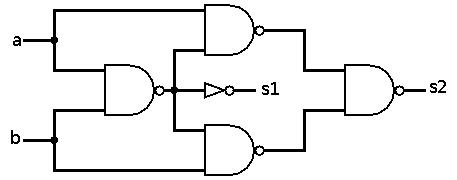
\includegraphics[scale=0.5]{Question6.jpg} 
\begin{flushleft}
$s_{1} = ab$\\
$s_{2} = \overline{\overline{(a\overline{(ab)})} \times \overline{(b\overline{(ab)})}}$\\
$s_{2} = a\overline{(ab)}+b\overline{(ab)}$\\
$s_{2} = a(\bar{a}+\bar{b}) + b(\bar{a}+\bar{b})$\\
$s_{2} = a\bar{a}+a\bar{b}+b\bar{a}+b\bar{b}$\\
$s_{2} = a\bar{b}+b\bar{a}$\\
$s_{1}$ est la fonction ET. $s_{2}$ est la fonction XOR.
\end{flushleft}

\subsection{Algèbre vers circuit logique}
Dessiner un circuit logique pour chacune des fonctions f et g de la partie précédente en utilisant unique des portes logiques (ET, OU, NON).

\subsubsection{$f(x,y,z) = xy+xz+yz$}
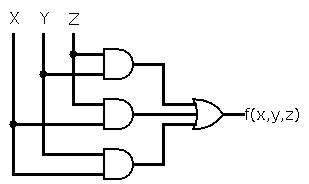
\includegraphics[scale=0.5]{Question7f.jpg} 

\subsubsection{$g(a,b,c) = \bar{a}\bar{b}\bar{c} + \bar{a}b\bar{c} + \bar{a}bc + a\bar{b}\bar{c} + ab\bar{c} + abc$}
$g(a,b,c) = \bar{a}\bar{b}\bar{c} + \bar{a}b+ a\bar{c} + abc$\\
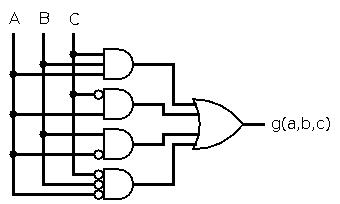
\includegraphics[scale=0.5]{Question7g.jpg} 

\section{Multiplexeur et démultiplexeur}
\subsection{Multiplexeur 2 vers 1}
\subsubsection{Table de vérité}
\begin{tabular}{ccc|c}
$e_{0}$ & $e_{1}$ & select & output \\ 
\hline 
0 & 0 & 0 & 0\\ 
0 & 1 & 0 & 0\\ 
1 & 0 & 0 & 1\\ 
1 & 1 & 0 & 1\\ 
0 & 0 & 1 & 0\\ 
0 & 1 & 1 & 1\\ 
1 & 0 & 1 & 0\\ 
1 & 1 & 1 & 1\\ 
\end{tabular} 

\subsubsection{Expression booléenne et circuit logique}
$o = e_{0}\bar{s} + e_{1}s$\\
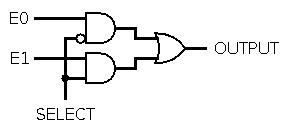
\includegraphics[scale=0.5]{mult2vers1.jpg} 

\subsection{Multiplexeur 4 vers 1}
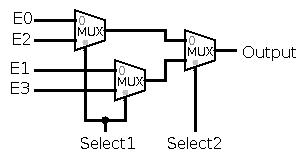
\includegraphics[scale=0.5]{mult4vers1_1.jpg}\\

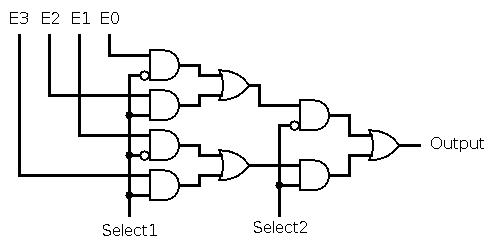
\includegraphics[scale=0.4]{mult4vers1_2.jpg}  

\subsection{Démultiplexeur 1 vers 4}
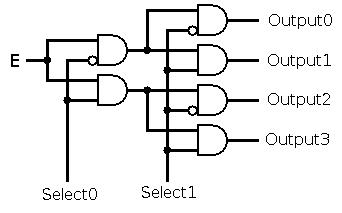
\includegraphics[scale=0.5]{demult1vers4.jpg} 

\newpage
\part{Circuits combinatoires}
\section{Additionneur 1 bit}
\subsection{Principe}
Un additionneur 1 bit est un circuit combinatoire à 3 entrées et deux sorties qui permet de réaliser l'addition de deux opérandes à 1 bit avec éventuellement une retenue en entrée sur 1 bit:
\begin{itemize}
\item 	Les entrées :
		\begin{itemize}
		\item a : entrée à 1 bit (opérande 1 de l'addition)
		\item b : entée à 1	bit (opérande 2 de l'addition)
		\item $c_{in}$ : retenue d'entrée de l'addition
		\end{itemize}
\item 	Les sorties :
		\begin{itemize}
		\item s : sortie à 1 bit résultat de l'addition
		\item $c_{out}$ : retenue de sortie de l'addition
		\end{itemize}
\end{itemize}

\subsection{table de vérité}
\begin{tabular}{ccc|cc}
a & b & $c_{in}$ & s & $c_{out}$ \\ 
\hline 
0 & 0 & 0 & 0 & 0 \\
0 & 0 & 1 & 1 & 0 \\
0 & 1 & 0 & 1 & 0 \\
0 & 1 & 1 & 0 & 1 \\
1 & 0 & 0 & 1 & 0 \\
1 & 0 & 1 & 0 & 1 \\
1 & 1 & 0 & 0 & 1 \\
1 & 1 & 1 & 1 & 1 \\
\end{tabular} \\

\begin{tabbing}
\hspace{7cm}\=\kill
 $s = \bar{a}\bar{b}c_{in}+\bar{a}b\bar{c_{in}}+a\bar{b}\bar{c_{in}}+abc_{in}$ \> $c_{out} = bc_{out}+ac_{out}+ab $ 
\end{tabbing} 
\subsection{Circuit combinatoire}
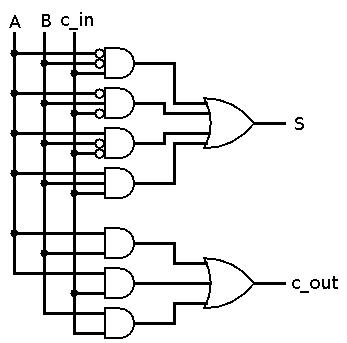
\includegraphics[scale=0.5]{Add1bit.jpg} 

\section{Additionneur 8 bits}
\subsection{Principe}
Un additionneur 8 bits est un circuit combinatoire à 3 entrées et deux sorties qui permet de réaliser l'addition de deux opérandes à 8 bits avec éventuellement une retenue en entrée sur 1 bit:
\begin{itemize}
\item 	Les entrées :
		\begin{itemize}
		\item a : entrée à 8 bit (opérande 1 de l'addition)
		\item b : entée à 8	bit (opérande 2 de l'addition)
		\item $c_{in}$ : retenue d'entrée de l'addition sur 1 bit
		\end{itemize}
\item 	Les sorties :
		\begin{itemize}
		\item s : sortie à 8 bits, résultat de l'addition
		\item $c_{out}$ : retenue de sortie de l'addition sur 1 bit
		\end{itemize}
\end{itemize}

\subsection{Réutilisation}
L'additionneur 8 bits revient à additionner chaque bit séparément avec le transfert des retenus d'un bit au suivant. On utilise donc l'additionneur 1 bit déjà réalisé pour créer celui-ci.

\subsubsection{Circuit combinatoire}
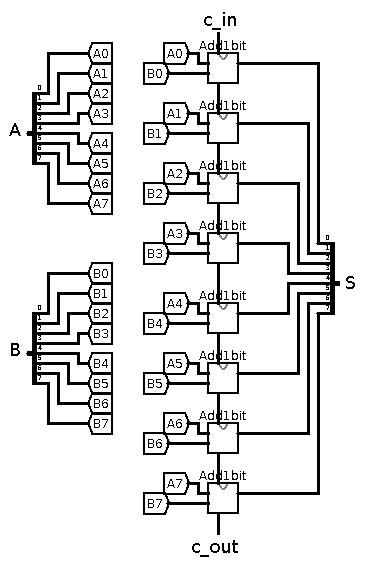
\includegraphics[scale=0.5]{Add8bit.jpg} 

\section{Additionneur/Soustracteur 8 bits}
\subsection{Principe}
La soustraction est en réalité extrêmement proche de l'addition. Elle revient à additionner l'opposé du nombre que l'on souhaite soustraire. Or en complément à 2 l'opposé est trouvé en prenant le complément du nombre (inverser tous les bits) et en ajoutant 1. On fait donc la différence entre un ordre d'addition et de soustraction par la valeur de la retenue d'entrée($c_{in}=0$ pour l'addition et $c_{in}=1$ pour la soustraction). Ensuite il suffit de prendre le complément de la $2^{ème}$ opérande pour la soustraction et on réutilise l'additionneur 8 bits.

\subsection{Inverseur}
\subsubsection{Principe}
L'inverseur est la partie du circuit qui doit inverser les bits de la deuxième opérande si l'on fait une soustraction et ne rien faire pour une addition

\begin{itemize}
\item 	Les entrées :
		\begin{itemize}
		\item b : entée à 8	bits (opérande 2 de l'addition/soustraction)
		\item $c_{in}$ : retenue d'entrée de l'addition/soustraction
		\end{itemize}
\item 	Les sorties :
		\begin{itemize}
		\item b' : sortie à 8 bit, opérande prête pour l'additionneur
		\end{itemize}
\end{itemize}

\subsubsection{table de vérité}
Chaque bit est indépendant donc on en représente qu'un seul.

\begin{tabular}{cc|c}
b & $c_{in}$ & b' \\ 
\hline 
0 & 0 & 0 \\ 
0 & 1 & 1 \\ 
1 & 0 & 1 \\ 
0 & 0 & 1 \\ 
\end{tabular} 
$\ \ \ \ \ \ \ b' = \bar{b}c_{in} + b\overline{c_{in}}$


\subsubsection{Circuit combinatoire}
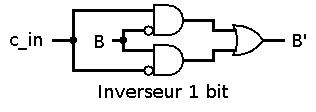
\includegraphics[scale=0.5]{Inverseur1bit.jpg}\\
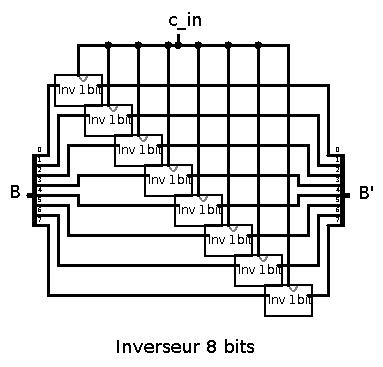
\includegraphics[scale=0.5]{Inverseur8bit.jpg}

\subsection{Implémentation Add/Sous 8 bits}
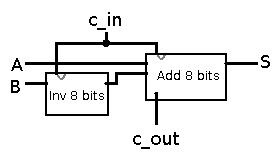
\includegraphics[scale=0.5]{AddSous8bits.jpg} 

\newpage
\part{Registres et mémoires}
\section{Registres}
\subsection{Latch et FlipFlop}
\subsubsection{Lactch ou verrou}
Le verrou permet de stocker une valeur quand l'entrée enable est à 0 et modifier cette velaur stockée quand enable est à 1. C'est un circuit séquentiel crée comme ceci:\\
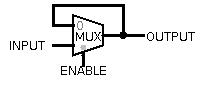
\includegraphics[scale=1]{Verrou.jpg} 

\subsubsection{Flip-Flop}
Le flip-flop permet de réaliser une bascule synchrone, c'est à dire que la sortie a toujours la valeur qu'avait l'entrée au dernier top d'horloge. Il est réalisé comme ci-dessous :\\
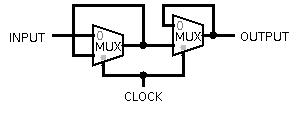
\includegraphics[scale=1]{FlipFlop.jpg} 

\subsection{Flip-Flop avec reset}
On complète le flip-flop avec un reset qui permet de remettre la sortie à 0 quelque soit l'entrée. Nous allons un réaliser un reset synchrone, cela signifie que la remise à 0 ne sera effective qu'à un top d'horloge. On doit donc avoir une entrée reset qui, quand elle est à 1, force l'entrée à 0.\\
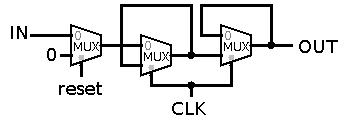
\includegraphics[scale=1]{FlipFlopReset.jpg} 

\subsection{Registre à commande de chargement}
La commande de chargement (communément appelé enable) permet de choisir quand on modifie ou non la valeur stockée. Pour ajouter cette commande au circuit précédent il suffit de "l'entourer" par le verrou vu juste au dessus :
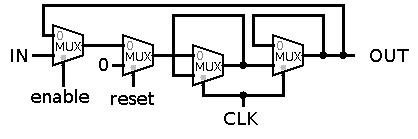
\includegraphics[scale=0.5]{registre1bit.jpg} 

\subsection{Registre à n bits}
Nous avons réussi à créer un registre complet à 1 bit. Pour la suite nous allons vouloir stocké beaucoup plus de valeur. Mais le travail est quasiment déjà fait puisqu'il nous suffit de mettre côte à côte autant de registre que l'on veut stocker de bits. Par exemple un registre 8 bits est fait ainsi:\\
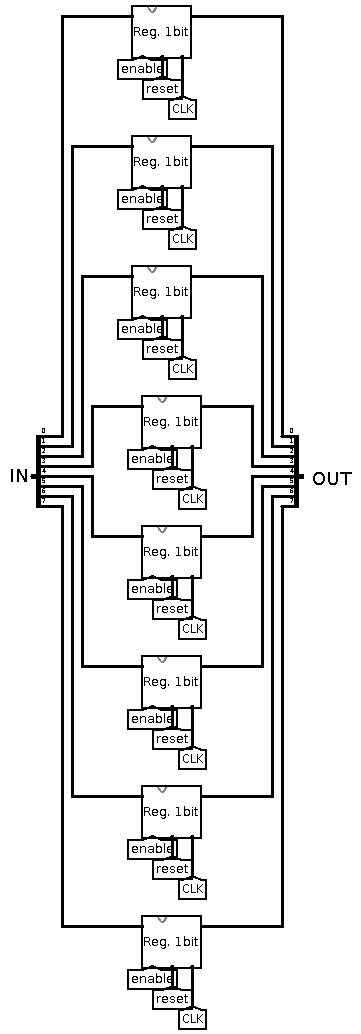
\includegraphics[scale=0.5]{registre8bits.jpg} 

\subsection{Un petit compteur}
Nous allons réaliser un circuit qui va compter les tops d'horloge dans un registre 8 bits. Le compteur peut aller de 0 à $2^{8}-1$\\
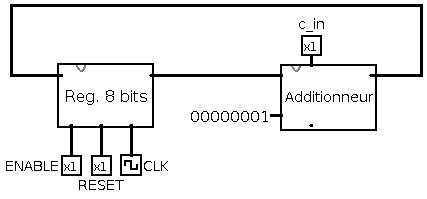
\includegraphics[scale=0.7]{Compteur.jpg} 

\section{Mémoires adressables}
\subsection{Démultiplexeur de 1 vers 8}
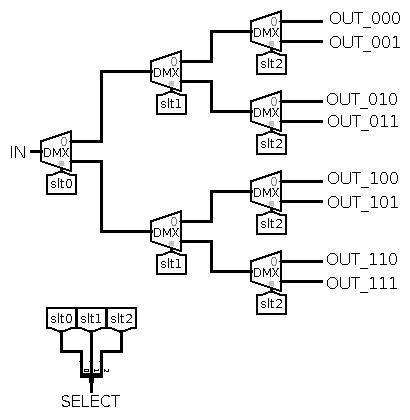
\includegraphics[scale=0.7]{Demux1vers8.jpg} 

\subsection{Multiplexeur de 8 vers 1}
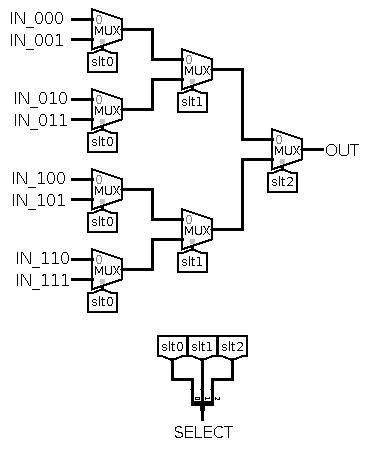
\includegraphics[scale=0.7]{Mux1vers8.jpg} 

\subsection{Mémoire 8 mots de 8 bits}
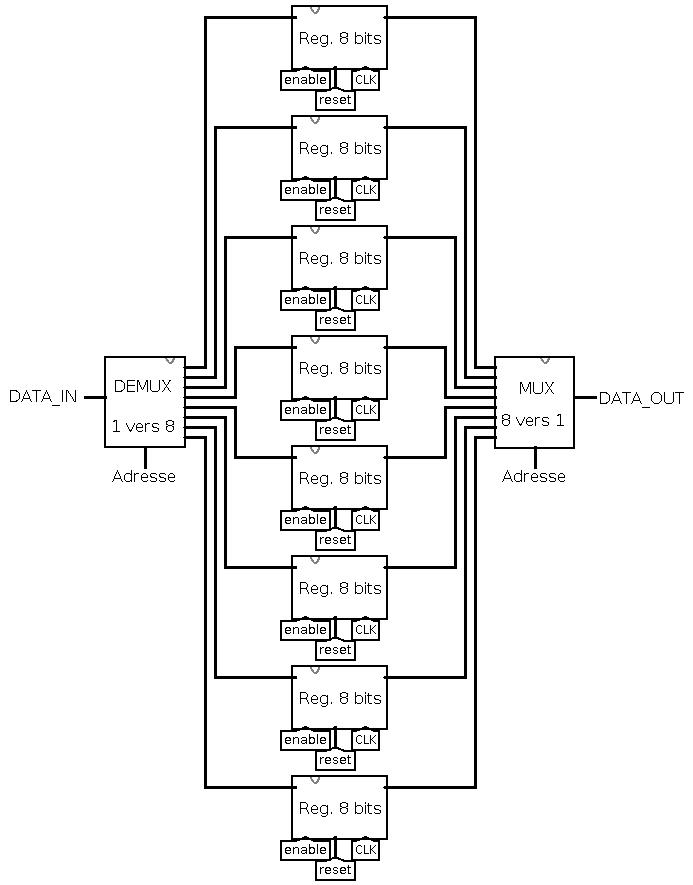
\includegraphics[scale=0.4]{Memoire.jpg} 


\newpage
\part{Automates}
\end{document}